\subsection{Dictionary}
\label{subsec:pd:dict}


% ----------------------- paths to graphics ------------------------

\graphicspath{{5_automatic_learning/pattern_detection/images/}}

% ----------------------- contents from here ------------------------
% 

We implemented a \textit{whitebox} version of Dictionary encoding to serve as a prior compression step before \nameref{subsec:pd:columncorrelation}. The pattern detector receives an additional parameter \(size_{max}\)---maximum size of the dictionary. We restricted its scope to \verb|VARCHAR| columns. This is a single-column pattern detector and columns are evaluated independently. The next paragraphs describe the pattern detection process for a single column.

Dictionary encoding only produces good results on columns that have a small number of unique values. However, it is hard to reliably quantify this property when analyzing only a sample of the data. Moreover, the distribution of unique values may be skewed, with only a few values with high frequency and a long tail of low frequency values. For the purpose of our pattern detector, we addressed this issue by enforcing a maximum dictionary size (in bytes) and only keeping the most common values in the dictionary. This approach is also suitable if blocks of data are compressed independently: dictionaries need to be small as they are assigned per block. There are other (possibly better) ways of optimizing the dictionary values and size. However, this is not a core aspect for our pattern detector, since we only use it as an intermediate step required for \nameref{subsec:pd:columncorrelation}.

The dictionary is built as follows. The \textit{scanning} phase creates the histogram of all the values in the sample. In the \textit{evaluation} step we select as many values (\(v_{s}\)) from the histogram---in decreasing order of their number of occurrences---such that their total size is smaller or equal to the maximum size of the dictionary (\(size_{max}\)). The dictionary is represented as an array containing the selected values. The indices in the array represent the dictionary ids (\(v_{id}\)) used to encode the values (\(v_{s}\)). The dictionary represents the compression and decompression metadata. All the values that are not present in the dictionary are considered exceptions.

The pattern detector only outputs results for columns that are dictionary compressible. This decision is taken based on the estimated size of the input column, output columns and metadata:
\begin{equation}
\label{eq:pd:dict:outputcondition}
    size_{in} > size_{out} + size_{ex} + size_{metadata}
\end{equation}
where:
\begin{itemize}
    \item[] \(size_{in}\) = estimated size of the input column
    \item[] \(size_{out}\) = estimated size of the dictionary ids column
    \item[] \(size_{ex}\) = estimated size of the exceptions column
    \item[] \(size_{metadata}\) = size of the dictionary
\end{itemize}

If the above condition is \textit{True}, the input column is considered dictionary compressible and the pattern detector outputs a result for it. More details about how these sizes are computed are given in \ref{subsub:estimator:dict}~\nameref{subsub:estimator:dict}. The \textit{evaluation result} is composed of the \textit{coverage} and \textit{row\_mask}---as defined in \ref{subsec:genericpd}~\nameref{subsec:genericpd}.

The \textit{expression nodes} for the \nameref{subsec:pd:dict} pattern are illustrated in Figure~\ref{fig:pd:dict:exprnode}.

\begin{figure}[h]
  \centering
  \begin{subfigure}[t]{0.4\linewidth}
    \centering
    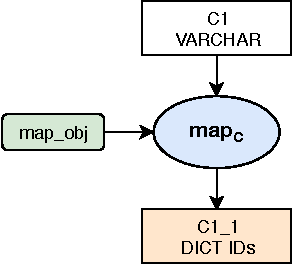
\includegraphics[width=0.8\linewidth]{expression_node-dictionary-compression_3.pdf}
    \caption[b]{compression}
    \label{fig:pd:dict:exprnode:compression}
  \end{subfigure}
  \hspace{1em}
  \begin{subfigure}[t]{0.4\linewidth}
    \centering
    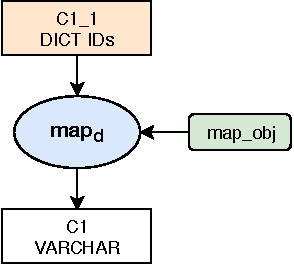
\includegraphics[width=0.8\linewidth]{expression_node-dictionary-decompression_3.pdf}
    \caption[b]{decompression}
    \label{fig:pd:dict:exprnode:decompression}
  \end{subfigure}
  \caption{Dictionary expression nodes}
  \label{fig:pd:dict:exprnode}
\end{figure}

The \textit{compression node} takes as input the string column and the dictionary \(map\_obj\). It outputs a column containing dictionary ids. The \textit{decompression node} takes as input the dictionary ids column and the dictionary and reconstructs the original input column.

The compression operator \(map_{c}\) takes as input the string value \(v_{s}\) and the dictionary \(map\_obj\) and outputs a dictionary id: the index of \(v_{s}\) in the array \(map\_obj\). As an optimization for the compression phase, \(map\_obj\) is represented as an actual dictionary with (\(v_{s}\), \(\mathit{index\_of}(v_{s})\)) key-value pairs instead of an array. If \(v_{s}\) is not found in \(map\_obj\) an \textit{OperatorException} is raised, indicating that \(v_{s}\) is an exception and should be stored in the exception column. The decompression operator \(map_{d}\) takes as input a dictionary id \(v_{id}\) (i.e. an index in the \(map\_obj\) array) and returns the original value \(v_{s}\) (\(map\_obj[v_{id}]\)).

% ---------------------------------------------------------------------------
% ----------------------- end of thesis sub-document ------------------------
% ---------------------------------------------------------------------------